% Title: gl2ps_renderer figure
% Creator: GL2PS 1.3.9, (C) 1999-2015 C. Geuzaine
% For: Octave
% CreationDate: Mon Nov 27 09:16:07 2017
\setlength{\unitlength}{1pt}
\begin{picture}(0,0)
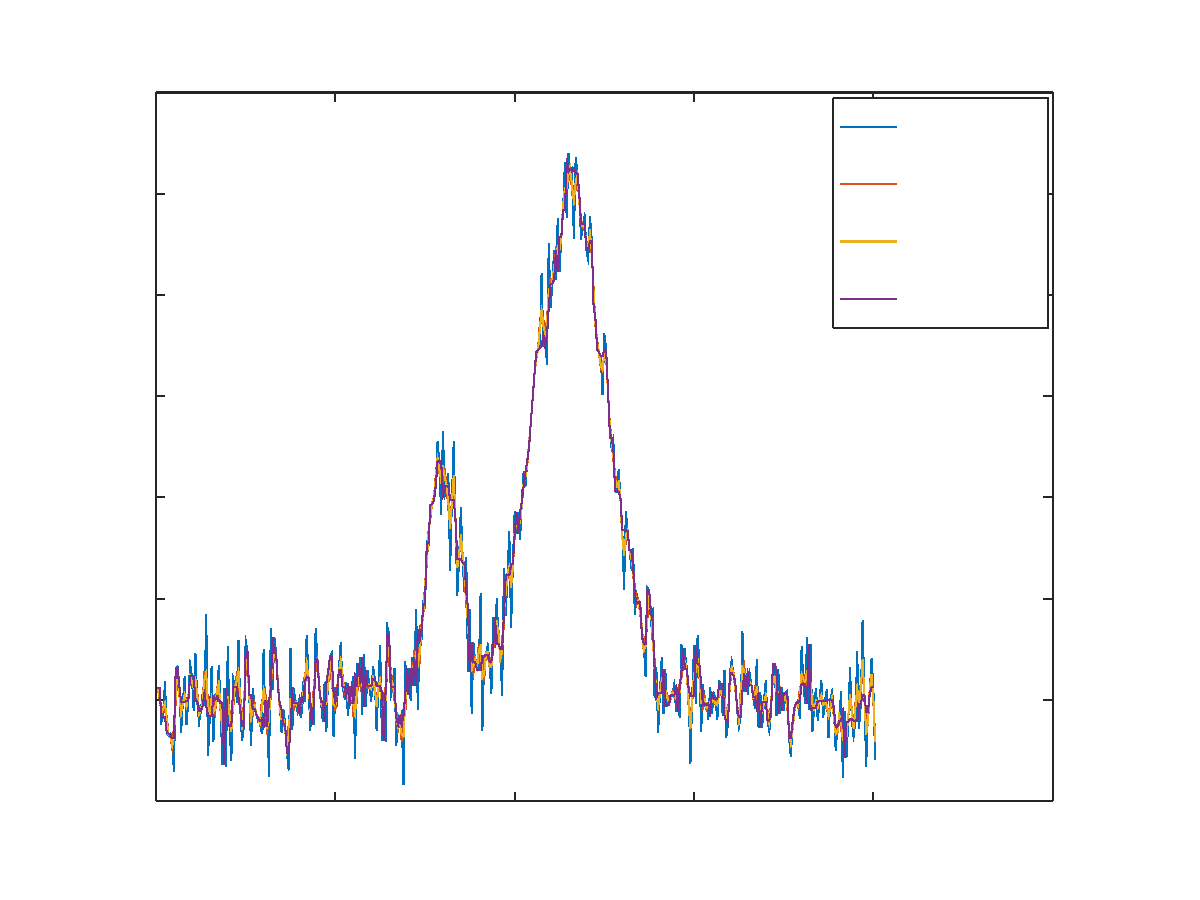
\includegraphics{low_pass_filters-inc}
\end{picture}%
\begin{picture}(576,432)(0,0)
\fontsize{12}{0}
\selectfont\put(74.88,42.5188){\makebox(0,0)[t]{\textcolor[rgb]{0.15,0.15,0.15}{{0}}}}
\fontsize{12}{0}
\selectfont\put(160.96,42.5188){\makebox(0,0)[t]{\textcolor[rgb]{0.15,0.15,0.15}{{100}}}}
\fontsize{12}{0}
\selectfont\put(247.04,42.5188){\makebox(0,0)[t]{\textcolor[rgb]{0.15,0.15,0.15}{{200}}}}
\fontsize{12}{0}
\selectfont\put(333.12,42.5188){\makebox(0,0)[t]{\textcolor[rgb]{0.15,0.15,0.15}{{300}}}}
\fontsize{12}{0}
\selectfont\put(419.2,42.5188){\makebox(0,0)[t]{\textcolor[rgb]{0.15,0.15,0.15}{{400}}}}
\fontsize{12}{0}
\selectfont\put(505.28,42.5188){\makebox(0,0)[t]{\textcolor[rgb]{0.15,0.15,0.15}{{500}}}}
\fontsize{12}{0}
\selectfont\put(69.8753,47.52){\makebox(0,0)[r]{\textcolor[rgb]{0.15,0.15,0.15}{{-1}}}}
\fontsize{12}{0}
\selectfont\put(69.8753,96.1029){\makebox(0,0)[r]{\textcolor[rgb]{0.15,0.15,0.15}{{0}}}}
\fontsize{12}{0}
\selectfont\put(69.8753,144.686){\makebox(0,0)[r]{\textcolor[rgb]{0.15,0.15,0.15}{{1}}}}
\fontsize{12}{0}
\selectfont\put(69.8753,193.269){\makebox(0,0)[r]{\textcolor[rgb]{0.15,0.15,0.15}{{2}}}}
\fontsize{12}{0}
\selectfont\put(69.8753,241.851){\makebox(0,0)[r]{\textcolor[rgb]{0.15,0.15,0.15}{{3}}}}
\fontsize{12}{0}
\selectfont\put(69.8753,290.434){\makebox(0,0)[r]{\textcolor[rgb]{0.15,0.15,0.15}{{4}}}}
\fontsize{12}{0}
\selectfont\put(69.8753,339.017){\makebox(0,0)[r]{\textcolor[rgb]{0.15,0.15,0.15}{{5}}}}
\fontsize{12}{0}
\selectfont\put(69.8753,387.6){\makebox(0,0)[r]{\textcolor[rgb]{0.15,0.15,0.15}{{6}}}}
\fontsize{12}{0}
\selectfont\put(290.08,397.6){\makebox(0,0)[b]{\textcolor[rgb]{0,0,0}{{Low-pass filters}}}}
\fontsize{12}{0}
\selectfont\put(433.703,371.177){\makebox(0,0)[l]{\textcolor[rgb]{0,0,0}{{$Y_{noise}$}}}}
\fontsize{12}{0}
\selectfont\put(433.703,343.628){\makebox(0,0)[l]{\textcolor[rgb]{0,0,0}{{$Y_{mean}$}}}}
\fontsize{12}{0}
\selectfont\put(433.703,316.08){\makebox(0,0)[l]{\textcolor[rgb]{0,0,0}{{$Y_{gaussian}$}}}}
\fontsize{12}{0}
\selectfont\put(433.703,288.531){\makebox(0,0)[l]{\textcolor[rgb]{0,0,0}{{$Y_{median}$}}}}
\end{picture}
